\documentclass[letterpaper,10pt]{article}

\usepackage{titling}
\usepackage{listings}
\usepackage{url}
\usepackage{setspace}
\usepackage{subfig}
\usepackage{sectsty}
\usepackage{pdfpages}
\usepackage{colortbl}
\usepackage{multirow}
\usepackage{relsize}
\usepackage{amsmath}
\usepackage{fancyvrb}
\usepackage{amsmath,amssymb,amsthm,graphicx,xspace}
\usepackage[titlenotnumbered,noend,noline]{algorithm2e}
\usepackage[compact]{titlesec}
\usepackage{paratype} 
\usepackage[T1]{fontenc}
\usepackage{tikz}
\usetikzlibrary{arrows,automata,shapes,trees,matrix,chains,scopes,positioning,calc}
\tikzstyle{block} = [rectangle, draw, fill=blue!20, 
    text width=2.5em, text centered, rounded corners, minimum height=2em]
\tikzstyle{bw} = [rectangle, draw, fill=blue!20, 
    text width=4em, text centered, rounded corners, minimum height=2em]

\definecolor{namerow}{cmyk}{.40,.40,.40,.40}
\definecolor{namecol}{cmyk}{.40,.40,.40,.40}

\let\LaTeXtitle\title
\renewcommand{\title}[1]{\LaTeXtitle{\textsf{#1}}}


\newcommand{\handout}[5]{
  \noindent
  \begin{center}
  \framebox{
    \vbox{
      \hbox to 5.78in { {\bf ECE254: Operating Systems and Systems Programming } \hfill #2 }
      \vspace{4mm}
      \hbox to 5.78in { {\Large \hfill #4  \hfill} }
      \vspace{2mm}
      \hbox to 5.78in { {\em #3 \hfill} }
    }
  }
  \end{center}
  \vspace*{4mm}
}

\newcommand{\lecture}[3]{\handout{#1}{#2}{#3}{Lecture #1}}
\newcommand{\tuple}[1]{\ensuremath{\left\langle #1 \right\rangle}\xspace}

\addtolength{\oddsidemargin}{-1.000in}
\addtolength{\evensidemargin}{-0.500in}
\addtolength{\textwidth}{2.0in}
\addtolength{\topmargin}{-1.000in}
\addtolength{\textheight}{1.75in}
\addtolength{\parskip}{\baselineskip}
\setlength{\parindent}{0in}
\renewcommand{\baselinestretch}{1.5}
\newcommand{\term}{Spring 2015}

\singlespace


\begin{document}

\lecture{ 1 --- Introduction to Operating Systems }{\term}{Jeff Zarnett}

\section*{About the Course}
We'll start by reviewing the highlights of the class syllabus. Please read it carefully (it is available in Learn under Content $\rightarrow$ Overview). It contains a lot of important information about the class including: the lecture topics, the grading scheme, contact information for the course staff, and university policies.

\section*{Introduction to Operating Systems}


\begin{quote}
\textit{Operating systems are those programs that interface the machine with the applications programs. The main function of these systems is to dynamically allocate the shared system resources to the executing programs.}

\textit{But the interface with adjacent levels continues to shift with
time. Functions that were originally part of the operating system have migrated to the hardware. On the other side, programmed functions extraneous to the problems being solved by the application programs are included in the operating system.
}
\end{quote}

\hfill - What Can Be Automated?: The Computer Science and Engineering Research Study, MIT Press, 1980

An operating system (often abbreviated OS) is a piece of software that sits between the hardware of a computer and the applications (programs) that run on that computer. The OS does many different things and often has many (occasionally-conflicting) goals. To use an analogy, you may wish to think of the operating system as the ``government'' of the computer: it is responsible for creating and enforcing the rules, providing an environment for other programs, and collecting and reporting data about what is and has been happening.

\begin{center}
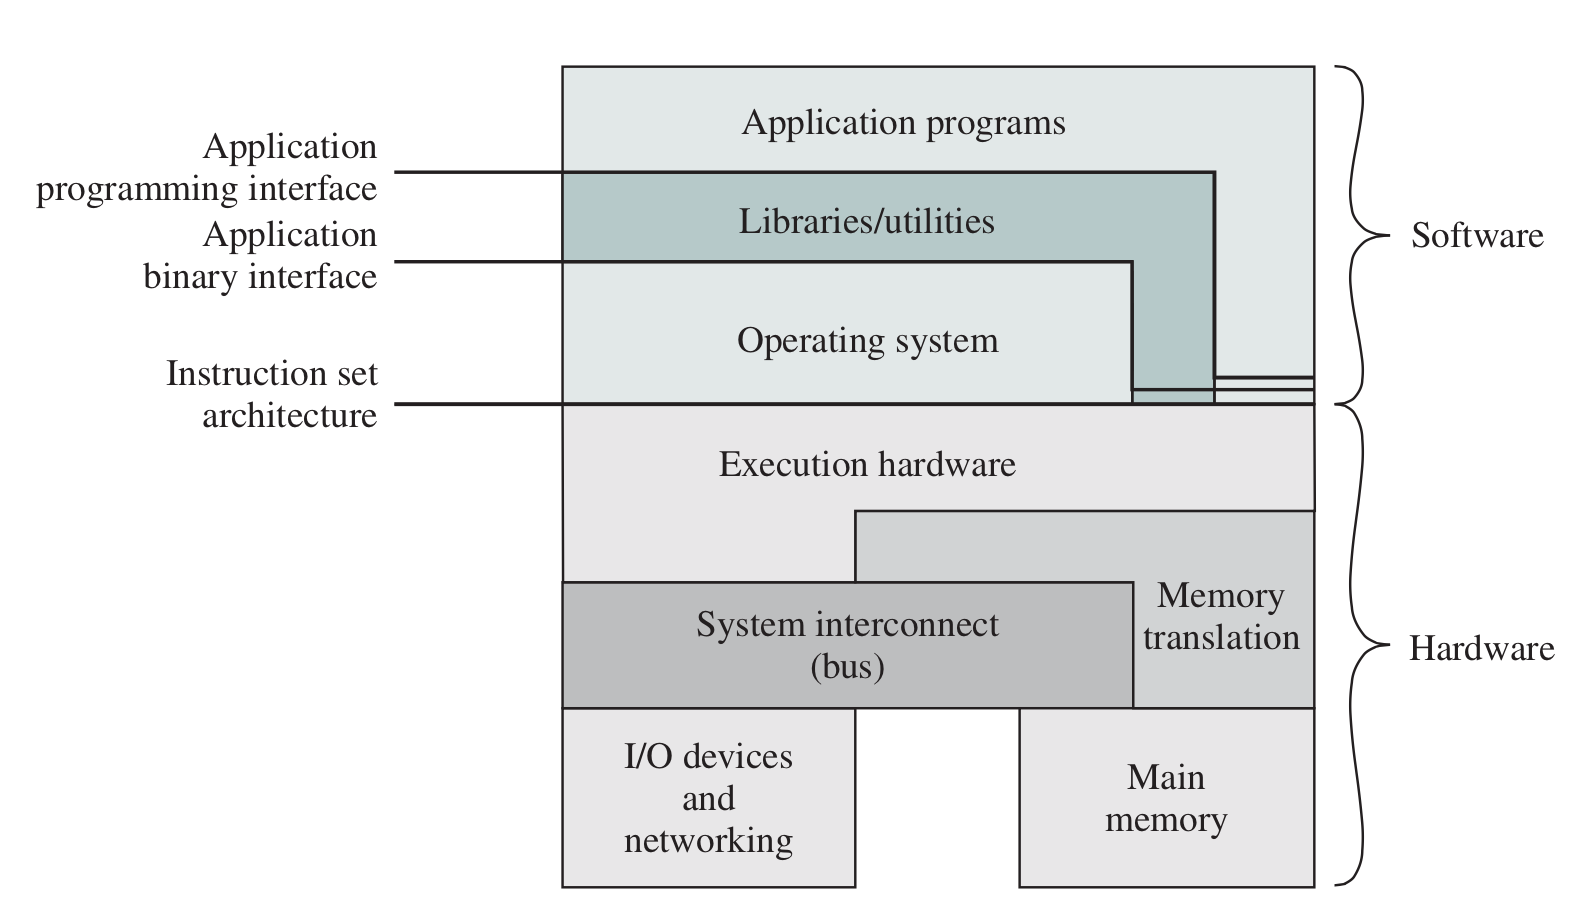
\includegraphics[width=0.75\textwidth]{images/os-sw-hw.png}\\
Structural diagram of a modern computer~\cite{osi}
\end{center}

An operating system is also responsible for resource allocation. In the real world, the resources we have to work with, such as CPU time or memory space, are limited. The OS decides how to allocate these resources, keeps track of who currently owns what, and, in the event of conflicting requests, determines who gets the resource.

The OS usually enables useful programs like Photoshop or Microsoft Word to run. Any computer has various pieces of hardware, such as the CPU, memory, input/output devices (such as monitors, keyboards, modems). The OS is responsible for abstracting away the details of this, so that the authors of programs do not have to worry about the specifics of the hardware. Imagine how painful it would be to write even a simple program, like the Hello World example, if we had to write our program differently for every combination of hardware.

In most cases there will be multiple programs running on the computer. This implies the sharing of various resources. When this is the case, there is the potential for conflicts to arise. An operating system creates and enforces rules to make sure all the programs get along and play fairly. Of course, not all interaction between programs is competitive; sometimes they want to co-operate, and the OS helps them do that, too.

Another goal may be to use the computer hardware efficiently. This is not usually an issue with personal laptops, but imagine a supercomputer. A supercomputer used to do extremely complex computations is expensive to build and maintain. Any moment when the supercomputer is not doing useful work is a costly waste, so an operating system for such a computer would try to maximize CPU usage. There is, after all, only so much CPU time in supercomputers and there are many programs eager to run (weather simulations, particle physics simulations...).

Operating systems tend to be large and do a lot of things. We expect now that an OS comes with a web browser, an e-mail client, some method for editing text, et cetera. These things, while important and useful, are not what we are going to focus on. The part of the operating system that we will study is what we call the \textit{Kernel} - it is the ``core''; the portion of the OS that is always present in main memory and the central part that makes it all work.

Operating systems will evolve over time. There will be new hardware released, new types of hardware, new services added, and bug fixes. Evolution is constrained by a need to maintain compatibility for programs. If the user upgrades his or her desktop OS and a program breaks, even if it's the program author's fault, the user blames the OS vendor. If you look at Microsoft Windows, you can see their strict devotion to not breaking binary compatibility (at least, as much as they reasonably can).

\subsection*{Systems Programming}
Operating systems themselves are not the whole picture; we also have to consider systems programming. This is the next layer above the operating system itself. System programs ship with the operating system and they are useful tools, but they are not part of the kernel. 

Some examples of things that might fall under systems programming (from~\cite{osc}):

\begin{itemize}
	\item \textbf{File Manipulation} - Programs to create, delete, copy, rename, print, and manipulate files and directories.
	\item \textbf{Status Information} - Monitor the state of the system for things like CPU usage, memory, disk space, etc.
	\item \textbf{Programming-Language Support} - Compilers and interpreters, including the command interpreter.
	\item \textbf{Communication} - Remote login capability, file transfer, download utilities, and messaging.
\end{itemize}

Programming at this level is more difficult than writing regular programs. It may require knowledge of the hardware, or perhaps programming facilities like debugging are limited. Furthermore, systems programs must take concurrency into account; multiple (regular) programs may try to use the systems program at the same time. An e-mail client may choose to refuse to allow two instances of the program to be open at the same time, but users would not accept a system that did not permit more than one file operation at a time. 

\section*{A Short History of Operating Systems}
Operating systems have evolved over the years, typically in conjunction with the hardware on which they run. We can put historical operating systems into various chronological ``buckets'', but the lines between the different categories are not so rigid. With that said, let us look at the categorization according to~\cite{mos}:

\paragraph{The Vacuum Tube Generation.} Way back in the 1940s and early 1950s, there were some devices recognizable as digital computers, but they did not have recognizable operating systems. Programming was done by wiring up the connections manually or perhaps connecting cables or flipping physical switches. One program could run at a time and figuring out whose turn it was followed a pretty simple process: there was a signup sheet where you could reserve a block of time. In the 1950s, however, there was a much better invention: the punch card!

\paragraph{The Second Generation.} From about 1955 to 1965 we had the era of the mainframe. Mainframes were extremely large (they filled very big rooms) and required a whole lot of professional operators to get them going. They were also so incredibly expensive, enough so that only government agencies, large corporations, and universities could afford them. Now to get some work done, the programmers create a ``job'', which is to say a program they have written out and then converted to punch cards. The programmer gives the deck of cards to an operator. The operator is responsible for inputting the cards and picking up the printout when it's done. 

At this point, there is an operating system, of a sorts: it is the operator who is responsible for managing each job. This is, however, a pretty inefficient operating system. To raise efficiency, the solution was the \textit{batch system}. In other words, group up a bunch of jobs and do them all together. This reduces the amount of time the mainframe is sitting around idle between jobs. While the mainframe is working on something else, have another (much more limited) system do the work of reading in the punch cards. Then when the mainframe is free, it gets a whole batch of jobs that are ready to run. Similarly, printing output can also be done by a limited system once the mainframe has finished a batch. 


\paragraph{The Third Generation.} From 1965-1980 it was the era of integrated circuits (ICs) and multiprogramming. As computers got better, IBM attempted to introduce the System/360, an operating system that was intended to run on multiple kinds of machine. IBM was making both high end (ones to do the heavy computing work) and low end computers (ones to do the boring jobs like printing) and they wanted one operating system to run on all their different hardware. This did not go well, prompting the writing of the book ``The Mythical Man-Month''~\cite{mmm}.\footnote{If you haven't read the book yet, you really should. If you took ECE~155 recently a good deal of the content of the book is represented in that course, but it's still worth reading. The book is short.} Nevertheless, IBM was on the right track: one of the things that makes operating systems like Windows, OS X, and Linux successful is that they work with whatever hardware you have (for the most part). 

These systems were still operating on the batch principle, done in such a way as to keep the CPU busy. In many older mainframes running things like military computations, the CPU was busy most of the time and was the limiting factor. In commercial applications, input/output (I/O) was often the limiting factor. Thus, it was ideal to have several jobs ready to go so the CPU's time would not be wasted. There was, however, a catch. Programmers submitted the job but it could take a long time to get back results. If the programmer made a mistake and got a compilation error, they might not find out until the next day. 

\begin{center}
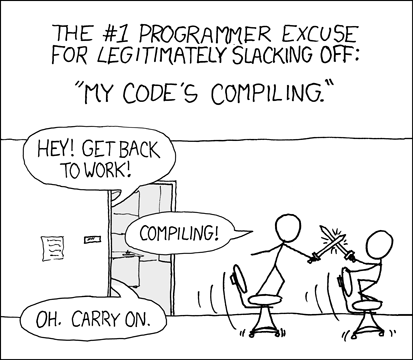
\includegraphics[width=0.45\textwidth]{images/compiling.png}\\
``My code's compiling.'' ~\cite{xkcd:compiling}
\end{center}

Thus, the next major innovation was \textit{timesharing} where each user gets a terminal connected to the central computer and users can enter commands. This allows for a more interactive and responsive system. Compilation might be quick if I am compiling a small block of code so getting results might not take very long. And while I am reading the output of the compiler (\texttt{SYNTAX ERROR LINE 5} is the way these things tend to look), the CPU can be working on something else: either some other user's interactive commands or a large batch job when there's nothing else to do. But this introduced a whole new problem because multiple programs are running at once: the various programs need to be protected from one another.

UNIX emerged in the third generation. The history of UNIX is long and varied, but it is arguably the most successful operating system ever. Almost all PC operating systems and many mobile ones are either descended from UNIX or an (often poor) attempt to reinvent it. The history and heritage of UNIX is long; too long to go over in this lecture. At this point it was possible to write programs to run on different systems so IEEE developed a standard, called \textit{POSIX} that versions of UNIX support. It turns out, humorously enough, that Windows NT is, in the most technical sense, POSIX-compliant, but Microsoft did the most minimal and nonfunctional implementation they could get away with for business reasons. Linux is a clone of UNIX intended to be compatible with and implement the POSIX standard.

\paragraph{The Fourth Generation.} Starting from about 1980, we entered the age of personal computers. In this era we saw the emergence of the IBM PC and the MS-DOS (MicroSoft Disk Operating System) and people having their own computers on their desks and in their homes. Up to this point interaction with the computer was all text based, until Apple capitalized on an invention by Xerox called the GUI (Graphical User Interface). We started to have operating systems that were user-friendly and not just for computer experts and programmers. Microsoft, of course, got the idea that it should have a GUI as well, and thus, Windows was born. UNIX users got a graphical interface too, called X11 (or X Windows). 

The GUI is more than just, if you will pardon the pun, window dressing. With the advent of the GUI a single user often started to have multiple things going on at a time, like playing some music while writing an essay with the e-mail program checking automatically for new mail. This is similar to the situation where we had multiple users all connected to the central system, in that protection between the various programs is needed. Parallelism receded for a while when people were using MS-DOS on their personal computers, but came back in a big way with Windows.

\paragraph{Wrapping Up.}
The history of the operating system of course is much more complex than this, but this is a very short overview of how we got to where we are. Much has changed in the era of the personal computer, but much has remained the same. The fundamental difficulties of using the hardware efficiently and protecting programs from one another have never gone away. The approaches we take to solve them are often very similar, if not identical, to the solutions devised in an earlier era.

As we proceed we will focus on UNIX-like systems with some mention of Microsoft Windows where appropriate. This is for practical reasons: there is only so much time and UNIX-like systems represent a very large percentage of the operating systems out there including Linux, Mac OS X, Android, and more. Windows, however, is quite different but noteworthy because of its widespread adoption. 

\bibliographystyle{alpha}
\bibliography{254}


\end{document}